% !TeX encoding = utf8
% !TeX program = pdflatex
% !TeXpellcheck = it_IT

\documentclass[a4paper,11pt,oneside]{article} 

\usepackage{relazioni}
\usepackage{imakeidx}
\usepackage{colortbl}
\usepackage{booktabs}
\usepackage{blindtext}
\usepackage{titletoc}
\usepackage{hyperref}
\usepackage{graphicx}
\usepackage{subcaption}
\usepackage{wrapfig}
\usepackage{geometry}
\usepackage{array}
\usepackage[export]{adjustbox}
\usepackage{multirow}
\usepackage{multicol}

\usepackage{colortbl}


\graphicspath{{Figure/}}
\DeclareSIUnit\micronnewton{\micro\metre\per\newton}




\begin{document}
\input{Front-matter/Frontespizio}

\tableofcontents
\addtocontents{toc}{~\hfill{Pagina}\par}
\contentsmargin{6em}
\dottedcontents{section}[1em]{\bigskip}{2em}{1pc}
\dottedcontents{subsection}[3em]{\smallskip}{3em}{1pc}
\dottedcontents{subsubsection}[5em]{\smallskip}{4em}{1pc}


\newpage

\section{Obiettivo}
L'obiettivo dell'esperienza è la verifica del comportamento elastico di un filo metallico, la stima del suo costante elastica $K$ e del relativo modulo di Young $E$.

\section{Apparato sperimentale}\label{section:apparato}

\begin{figure}[h!]
    \centering
    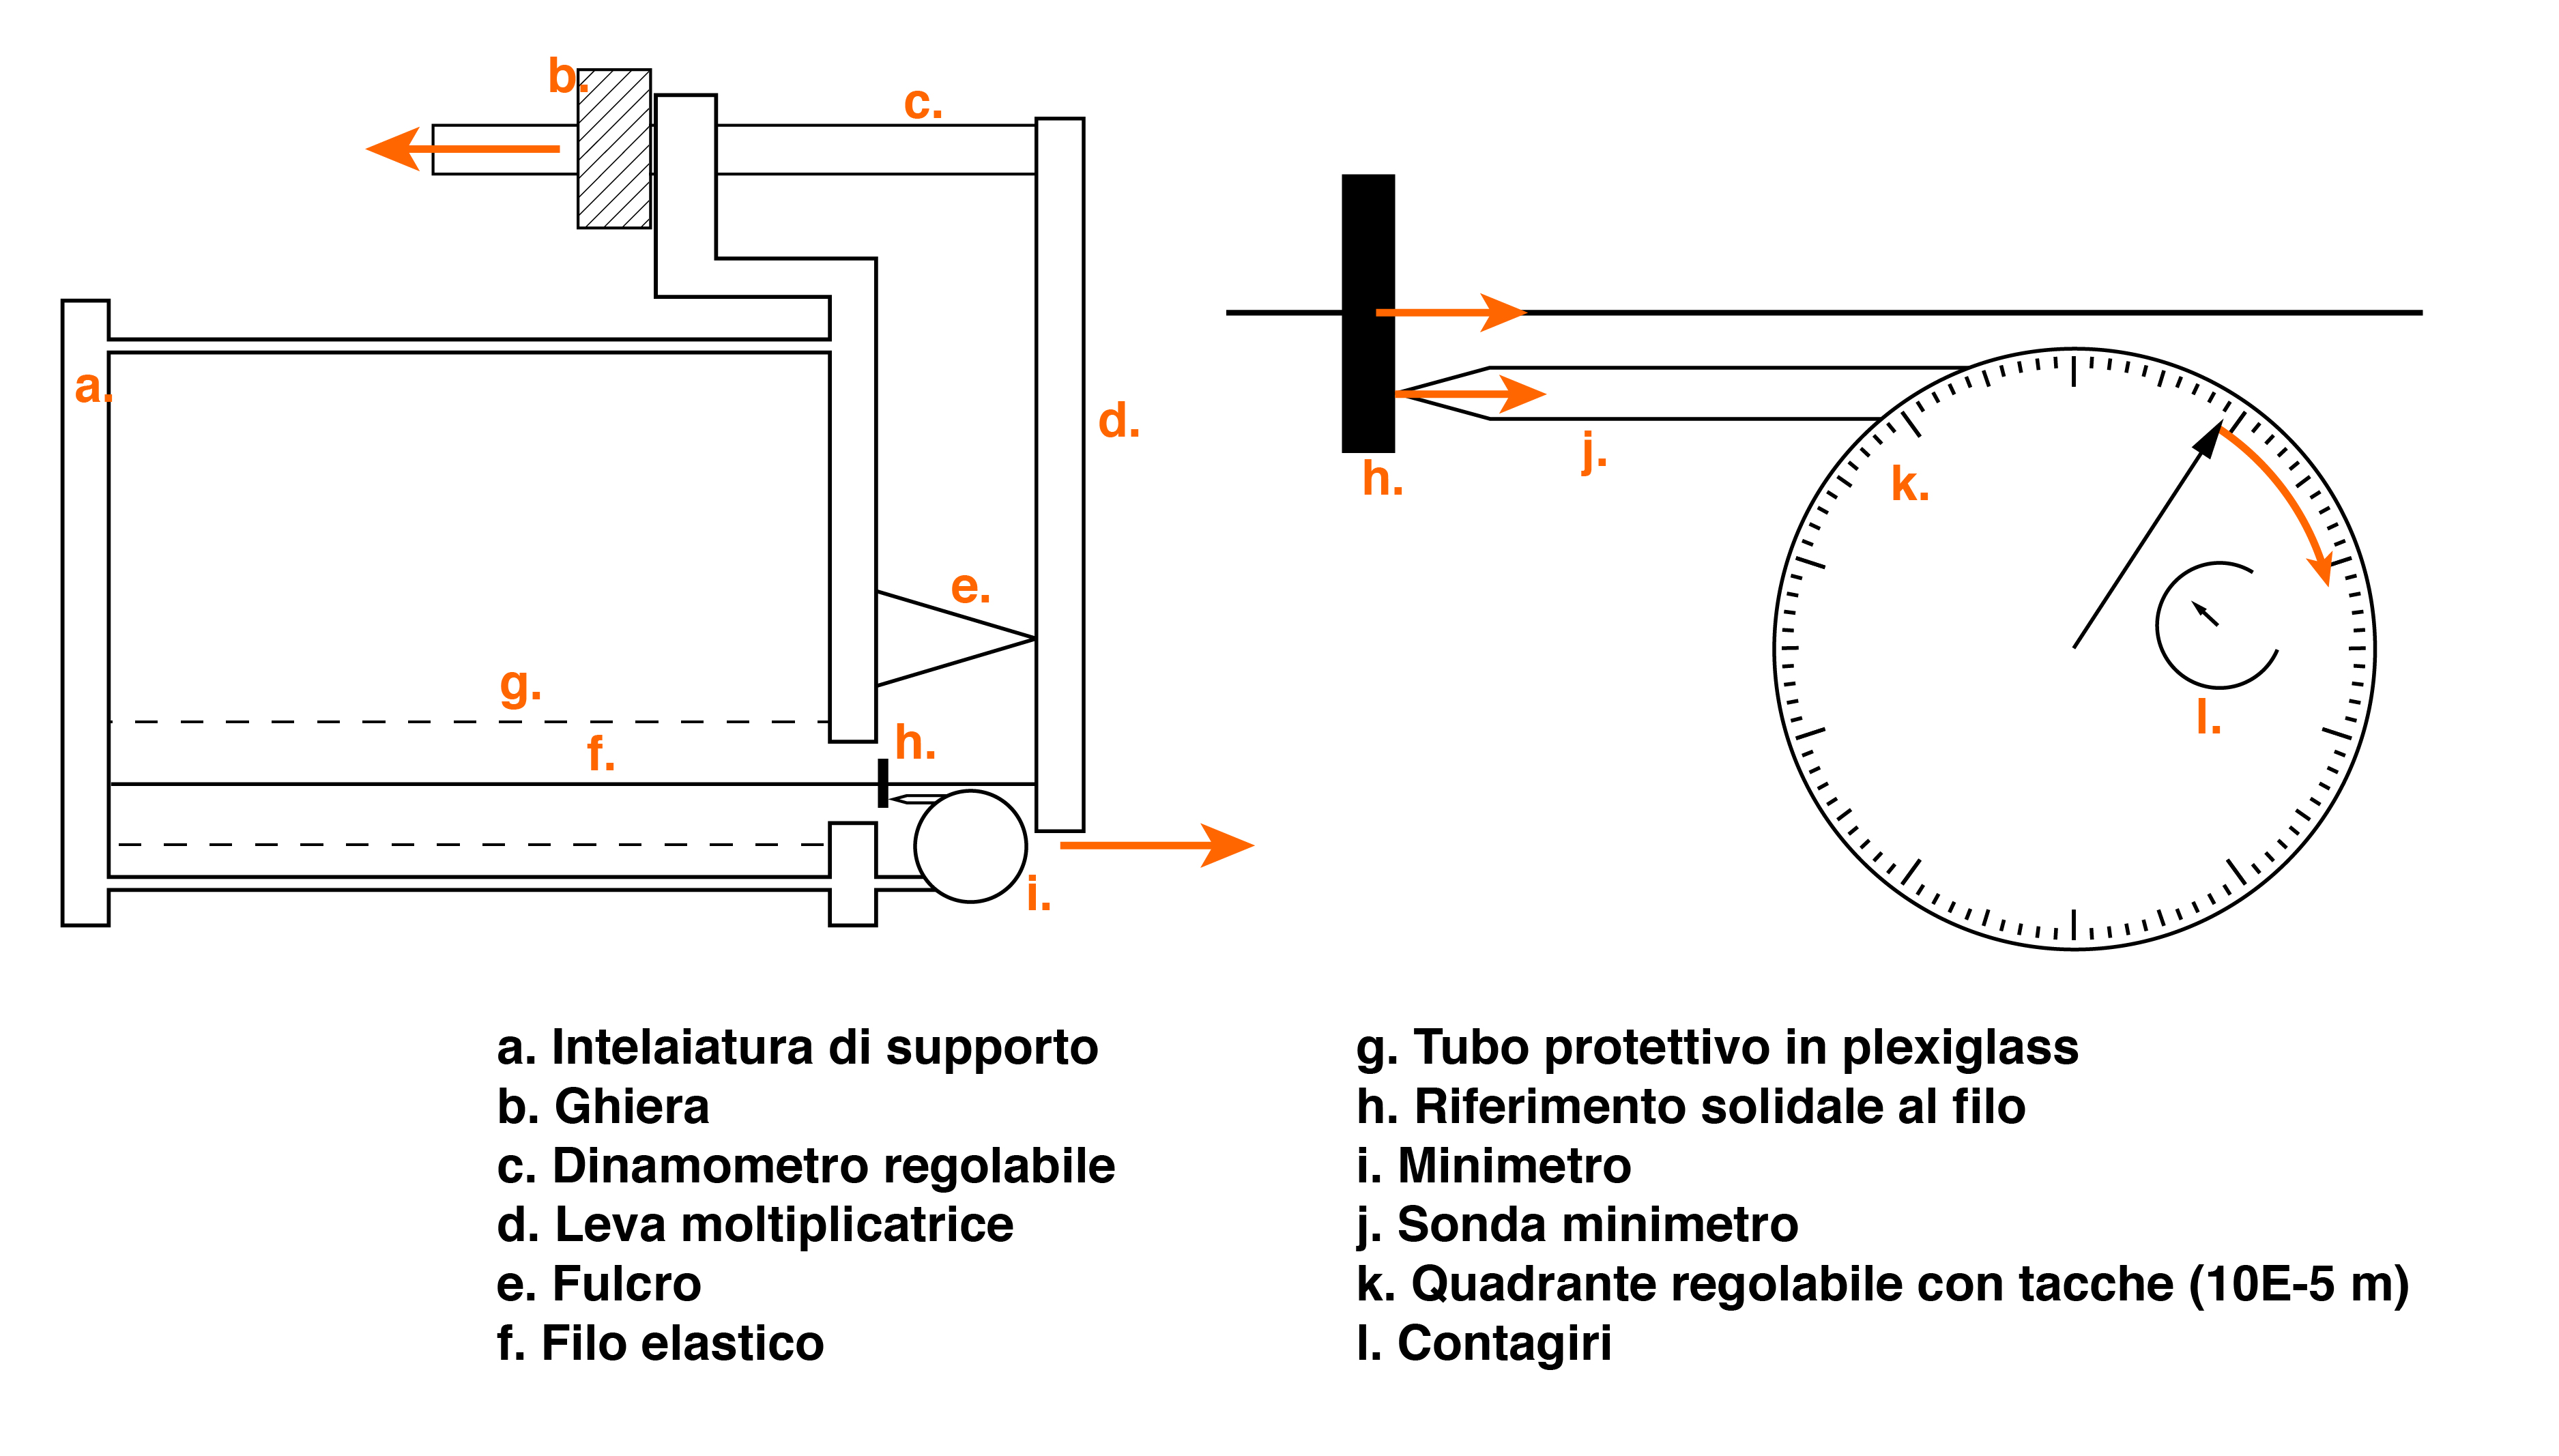
\includegraphics[width=12.5cm]{ApparatoSperimentale.jpg}
    \caption{Diagramma composizione apparato sperimentale}
    \label{fig:apparato_sperimentale}
\end{figure}
L'apparato sperimentale risulta così composto:
\begin{enumerate}
    \item Un cilindro metallico (acciaio, tungsteno o ottone) posto internamente ad un tubo protettivo a tutela di perturbazioni esterne. Lo stesso ha un'estremità fissata in maniera solidale alla struttura di supporto e nella parte finale presenta un disco forato, al fine di valutarne l'allungamento.
    \item Un minimetro a quadrante regolabile con sensibilità $S=\num{1e5} \si{m^{-1}}$ con sonda appoggiata al riferimento. E' presente inoltre un contatore interno al quadrante del minimetro che tiene conto dei giri completi compiuti dalla lancetta.
    \item Un dinamometro regolabile tramite una ghiera che, ruotando, varia la forza applicata al filo. L'unità di misura utilizzata è grammi peso, avente la più piccola tacca di lettura pari $\SI{100}{gp}$
    \item Una leva collegata al filo metallico e al dinamometro utilizzata per quadruplicare la forza esercitata dal dinamometro.
\end{enumerate}
Nel complesso sono stati impiegati 12 estensimetri diversi, dei quali vengono riassunte le caratteristiche nella Tabella \ref{tab:caratteristiche_estensimetri}.

\begin{table}[h!]
	\centering
	\begin{tabular}{|l|c|c|c|}  
\hline
		    Materiale & \#& \multicolumn{1}{l}{Lunghezza}        & \multicolumn{1}{l}{Diametro}\\ 
		    &&$[\si{mm}] \pm\SI{2}{mm}$&$[\si{mm}] \pm\SI{1}{\percent}$\\  
\hline
\multirow{9}{*}{Acciaio} & {\cellcolor[rgb]{0.753,0.753,0.753}}1  & {\cellcolor[rgb]{0.753,0.753,0.753}}950  & {\cellcolor[rgb]{0.753,0.753,0.753}}0.33   \\
& 2 & 950 & 0.356  \\
& {\cellcolor[rgb]{0.753,0.753,0.753}}3  & {\cellcolor[rgb]{0.753,0.753,0.753}}950  & {\cellcolor[rgb]{0.753,0.753,0.753}}0.381  \\
& 4 & 950 & 0.305  \\ & {\cellcolor[rgb]{0.753,0.753,0.753}}5  & {\cellcolor[rgb]{0.753,0.753,0.753}}950  & {\cellcolor[rgb]{0.753,0.753,0.753}}0.3    \\
& 6 & 950 & 0.4                                        \\
& {\cellcolor[rgb]{0.753,0.753,0.753}}7  & {\cellcolor[rgb]{0.753,0.753,0.753}}950  & {\cellcolor[rgb]{0.753,0.753,0.753}}0.279  \\
& 8 & 600 & 0.279                                      \\
& {\cellcolor[rgb]{0.753,0.753,0.753}}9  & {\cellcolor[rgb]{0.753,0.753,0.753}}800  & {\cellcolor[rgb]{0.753,0.753,0.753}}0.279  \\
& 10 & 700 & 0.279                                      \\
\hline
Tungsteno & {\cellcolor[rgb]{0.753,0.753,0.753}}11 &{\cellcolor[rgb]{0.753,0.753,0.753}} 1000 &{\cellcolor[rgb]{0.753,0.753,0.753}} 0.25\\
\hline
Ottone                   & 12 & 1000 & 0.5\\ \hline
\end{tabular}
	\caption{Estensimetri impiegati}
	\label{tab:caratteristiche_estensimetri}
\end{table}



\section{Metodi acquisizione dati}
Si specifica che i dati relativi alla prima parte sono stati trascritti da registrazioni video dell'apparato sperimentale composto dal decimo estensimetro. I dati impiegati nell'analisi sistematica dei vari estensimetri sono invece stati direttamente forniti in tabelle.\\

Vengono qui esposti i due diversi metodi impiegati per raccogliere i dati nella prima parte.

\subsection{Primo metodo - Allungamento e Accorciamento}%aumento di 100 in 100
Come operazione preliminare si è agito sulla ghiera dell'estensimetro, manovrandola in modo tale che segnasse una tensione $F_{letta}=\SI{200}{gp}$ così da mettere in tensione il filo di metallo analizzato. Si è poi sollecitata delicatamente la manopola della sonda del minimetro così da eliminare l'eventuale contributo di giochi meccanici ed infine si è impostata la ghiera del minimetro in modo che lo zero del quadrante coincidesse con la posizione della lancetta maggiore. Dopo aver annotato il valore letto sul minimetro, tendendo in considerazione che una rotazione completa della lancetta corrisponde una variazione di lunghezza pari a $\num{1} \si{mm}$, si è manovrata la ghiera del dinamometro portandola alla tacca successiva, ovvero aumentando la forza letta di $\SI{100}{gp}$. Avendo cura di non oltrepassare la tacca e di smuovere la manopola della sonda di volta in volta, si sono annotati tutti i valori segnati dal minimetro. La ghiera è stata manovrata fino ad arrivare ad una forza letta di $\SI{1200}{gp}$. A tal punto si è diminuita la tensione esercitata dal dinamometro, variando sempre la $F_{letta}$ di $\SI{100}{gp}$, e annotando i valori del minimetro.\\

\subsection{Secondo metodo - Misure ripetute}%video 400 -1000
Riportato l'estensimetro con il dinamometro a $\SI{200}{gp}$ si sono eseguite misure ripetute. La procedura è consistita nel portare il dinamometro ad esercitare una tensione letta di $\SI{400}{gp}$, dapprima aumentandola a partire da $\SI{200}{gp}$, poi diminuendola a partire da $\SI{600}{gp}$. È stata prestata la massima attenzione nel non oltrepassare la tacca di $\SI{400}{gp}$.
Il procedimento è stato effettuato per 9 volte "in accorciamento" e 8 "in allungamento" in corrispondenza della tacca $\SI{400}{gp}$ per poi ripetere la presa dati in corrispondenza della tacca di $\SI{1000}{gp}$, variando "in accorciamento" fino a $\SI{800}{gp}$ e "in allungamento" fino a $\SI{1200}{gp}$.\\
E' opportuno precisare che l'analisi dei video è stata compiuta singolarmente: ogni operatore ha trascritto la lettura del minimetro corrispondente ad ogni misurazione, in modo da avere un campione più significativo e compiere una analisi statistica più accurata.

%POSSIBILE INSERIMENTO DI HEADER TABELLE SADA PER COMPLETEZZA

\section{Analisi dati}
%INTRO GENERICA
Nella prima parte l'analisi si è svolta esclusivamente sull'estensimetro numero 10 riportato in Tabella \ref{tab:caratteristiche_estensimetri}. Nella seconda parte invece si è svolta un'analisi sistematica su tutti gli estensimetri in acciaio.

\subsection{Verifica dell'elasticità meccanica e definizione miglior protocollo di misura}\label{sec:prima_parte}
Sono stati impiegati diversi metodi per il calcolo del coefficiente elastico del filo del decimo estensimetro a seconda del metodo di raccolta dati.\\

\subsubsection*{Primo Metodo - Misure in allungamento e accorciamento}
\begin{table}[h!]
    \centering
    \begin{tabular}{|cc|c|c|c||c|c|c|}
        \hline
        & $F_{letta}$ & $\Delta x_{Op 1}$ & $\Delta x_{Op 2}$ &$ \Delta x_{Op 3}$ &$\overline{ \Delta x}$ & $\sigma_{\Delta x}$ & $\sigma_{\overline{\Delta x}}$\\ 
        & $[\si{gp}]$& $[\SI{e-6}{\meter}] $&$[\SI{e-6}{\meter}] $&$[\SI{e-6}{\meter}] $&$[\SI{e-6}{\meter}] $&$[\SI{e-6}{\meter}] $&$[\SI{e-6}{\meter}] $\\
        \hline
        \multicolumn{1}{|c|}{\multirow{11}{*}{\rotatebox[origin=c]{90}{Allungamento}}} & {\cellcolor[rgb]{0.85,0.85,0.85}}200&	{\cellcolor[rgb]{0.85,0.85,0.85}}-2&	{\cellcolor[rgb]{0.85,0.85,0.85}}-3&	{\cellcolor[rgb]{0.85,0.85,0.85}}-2&	{\cellcolor[rgb]{0.85,0.85,0.85}}-2,33333&	{\cellcolor[rgb]{0.85,0.85,0.85}}0,57735&	{\cellcolor[rgb]{0.85,0.85,0.85}}0,333333\\
        \multicolumn{1}{|c|}{}&300&	223&	222&	225&	223,333&	1,52753&	0,881917\\
        \multicolumn{1}{|c|}{}&{\cellcolor[rgb]{0.85,0.85,0.85}}400&	{\cellcolor[rgb]{0.85,0.85,0.85}}431&	{\cellcolor[rgb]{0.85,0.85,0.85}}431&	{\cellcolor[rgb]{0.85,0.85,0.85}}430&	{\cellcolor[rgb]{0.85,0.85,0.85}}430,667&	{\cellcolor[rgb]{0.85,0.85,0.85}}0,57735&	{\cellcolor[rgb]{0.85,0.85,0.85}}0,333333\\
        \multicolumn{1}{|c|}{}&500&	660&	660&	660&	660&	0&	0\\
        \multicolumn{1}{|c|}{}&{\cellcolor[rgb]{0.85,0.85,0.85}}600&	{\cellcolor[rgb]{0.85,0.85,0.85}}876&	{\cellcolor[rgb]{0.85,0.85,0.85}}878&	{\cellcolor[rgb]{0.85,0.85,0.85}}877&	{\cellcolor[rgb]{0.85,0.85,0.85}}877&	{\cellcolor[rgb]{0.85,0.85,0.85}}1&	{\cellcolor[rgb]{0.85,0.85,0.85}}0,57735\\
        \multicolumn{1}{|c|}{}&700&	1093&	1091&	1092&	1092&	1&	0,57735\\
        \multicolumn{1}{|c|}{}&{\cellcolor[rgb]{0.85,0.85,0.85}}800&	{\cellcolor[rgb]{0.85,0.85,0.85}}1310&	{\cellcolor[rgb]{0.85,0.85,0.85}}1311&	{\cellcolor[rgb]{0.85,0.85,0.85}}1310&	{\cellcolor[rgb]{0.85,0.85,0.85}}1310,33&	{\cellcolor[rgb]{0.85,0.85,0.85}}0,57735&	{\cellcolor[rgb]{0.85,0.85,0.85}}0,333333\\
        \multicolumn{1}{|c|}{}&900&	1513&	1512&	1512&	1512,33&	0,57735&	0,333333\\
        \multicolumn{1}{|c|}{}&{\cellcolor[rgb]{0.85,0.85,0.85}}1000&	{\cellcolor[rgb]{0.85,0.85,0.85}}1749&	{\cellcolor[rgb]{0.85,0.85,0.85}}1749&	{\cellcolor[rgb]{0.85,0.85,0.85}}1748&	{\cellcolor[rgb]{0.85,0.85,0.85}}1748,67&	{\cellcolor[rgb]{0.85,0.85,0.85}}0,57735&	{\cellcolor[rgb]{0.85,0.85,0.85}}0,333333\\
        \multicolumn{1}{|c|}{}&1100&	1948&	1949&	1948&	1948,33&	0,57735&	0,333333\\
        \multicolumn{1}{|c|}{}&{\cellcolor[rgb]{0.85,0.85,0.85}}1200&	{\cellcolor[rgb]{0.85,0.85,0.85}}2170&	{\cellcolor[rgb]{0.85,0.85,0.85}}2170&	{\cellcolor[rgb]{0.85,0.85,0.85}}2170&	{\cellcolor[rgb]{0.85,0.85,0.85}}2170&	{\cellcolor[rgb]{0.85,0.85,0.85}}0&	{\cellcolor[rgb]{0.85,0.85,0.85}}0\\ 
        \hline\hline
        \multicolumn{1}{|c|}{\multirow{11}{*}{\rotatebox[origin=c]{90}{Allungamento}}} & {\cellcolor[rgb]{0.85,0.85,0.85}}1200&	{\cellcolor[rgb]{0.85,0.85,0.85}}2170&	{\cellcolor[rgb]{0.85,0.85,0.85}}2170&	{\cellcolor[rgb]{0.85,0.85,0.85}}2170&	{\cellcolor[rgb]{0.85,0.85,0.85}}2170,0&	{\cellcolor[rgb]{0.85,0.85,0.85}}0,0&	{\cellcolor[rgb]{0.85,0.85,0.85}}0,0\\
        \multicolumn{1}{|c|}{}&1100&	1949&	1950&	1950&	1949,7&	0,6&	0,3\\
        \multicolumn{1}{|c|}{}&{\cellcolor[rgb]{0.85,0.85,0.85}}1000&	{\cellcolor[rgb]{0.85,0.85,0.85}}1727&	{\cellcolor[rgb]{0.85,0.85,0.85}}1727&	{\cellcolor[rgb]{0.85,0.85,0.85}}1727&	{\cellcolor[rgb]{0.85,0.85,0.85}}1727,0&	{\cellcolor[rgb]{0.85,0.85,0.85}}0,0&	{\cellcolor[rgb]{0.85,0.85,0.85}}0,0\\
        \multicolumn{1}{|c|}{}&900&	1514&	1513&	1514&	1513,7&	0,6&	0,3\\
        \multicolumn{1}{|c|}{}&{\cellcolor[rgb]{0.85,0.85,0.85}}800&	{\cellcolor[rgb]{0.85,0.85,0.85}}1303&	{\cellcolor[rgb]{0.85,0.85,0.85}}1303&	{\cellcolor[rgb]{0.85,0.85,0.85}}1305&	{\cellcolor[rgb]{0.85,0.85,0.85}}1303,7&	{\cellcolor[rgb]{0.85,0.85,0.85}}1,2&	{\cellcolor[rgb]{0.85,0.85,0.85}}0,7\\
        \multicolumn{1}{|c|}{}&700&	1082&	1081&	1082&	1081,7&	0,6&	0,3\\
        \multicolumn{1}{|c|}{}&{\cellcolor[rgb]{0.85,0.85,0.85}}600&	{\cellcolor[rgb]{0.85,0.85,0.85}}869&	{\cellcolor[rgb]{0.85,0.85,0.85}}869&	{\cellcolor[rgb]{0.85,0.85,0.85}}869&	{\cellcolor[rgb]{0.85,0.85,0.85}}869,0&	{\cellcolor[rgb]{0.85,0.85,0.85}}0,0&	{\cellcolor[rgb]{0.85,0.85,0.85}},0\\
        \multicolumn{1}{|c|}{}&500&	655&	655&	655&	655,0&	0,0&	0,0\\
        \multicolumn{1}{|c|}{}&{\cellcolor[rgb]{0.85,0.85,0.85}}400&	{\cellcolor[rgb]{0.85,0.85,0.85}}430&	{\cellcolor[rgb]{0.85,0.85,0.85}}431&	{\cellcolor[rgb]{0.85,0.85,0.85}}430&	{\cellcolor[rgb]{0.85,0.85,0.85}}430,3&	{\cellcolor[rgb]{0.85,0.85,0.85}}0,6&	{\cellcolor[rgb]{0.85,0.85,0.85}}0,3\\
        \multicolumn{1}{|c|}{}&300&	219&	220&	220&	219,7&	0,6&	0,3\\
        \multicolumn{1}{|c|}{}&{\cellcolor[rgb]{0.85,0.85,0.85}}200&	{\cellcolor[rgb]{0.85,0.85,0.85}}2&	{\cellcolor[rgb]{0.85,0.85,0.85}}1&	{\cellcolor[rgb]{0.85,0.85,0.85}}2&	{\cellcolor[rgb]{0.85,0.85,0.85}}1,7&	{\cellcolor[rgb]{0.85,0.85,0.85}}0,6&	{\cellcolor[rgb]{0.85,0.85,0.85}}0,3\\
        \hline
    \end{tabular}
    \caption{Dati Grezzi con $\overline{\Delta x}$, $\sigma_{\Delta x}$, $\sigma_{\overline{\Delta x}}$}
    \label{tab:dati_grezzi_1ac}
\end{table}

Ogni operatore ha acquisito indipendentemente le misurazioni lette sul minimetro. Per ciascuna misurazione ad assetto analogo ($F_{app}$ e fase di allungamento o accorciamento) si sono computati i valori di $\overline{\Delta x}$, $\sigma_{\Delta x}$, $\sigma_{\overline{\Delta x}}$ (Tabella \ref{tab:dati_grezzi_1ac}).
%Per la prima acquisizione dati si è scelto di calcolare separatamente due diversi valori di K, mantenendo separati i dati raccolti quando il filo veniva allungato e quando il filo veniva accorciato. Si è utilizzato il metodo del minimo $\chi^2$ al fine di calcolare il coefficiente elastico, sfruttando la relazione lineare che lega l'allungamento o l'accorciamento del filo con la forza applicata per metterlo in tensione. La relazione è la seguente e prende il nome di legge di Hooke:
%\begin{equation*}
%       \left | x_i - x_0  \right |  = K \cdot  \left | F_i - F_0 \right |
%\end{equation*}
Il calcolo di $\sigma_{\overline{\Delta x}}$ rivela la presenza di errori nulli, pertanto al fine di non sottostimare l'errore sulla singola misura si è valutata opportunamente $\sigma_{\overline{\Delta x}}$ in confronto a $\sigma_{Dist. uni.}$, errore dalla distribuzione uniforme, in modo da utilizzare la stima più appropriata. I parametri della distribuzione uniforme risultano essere: $PTL= \SI{10}{micron}$ e $\text{Coeff. aff.}=\num{10}$.\\
Il confronto fra $\sigma_{\overline{\Delta x}}$ e $\sigma_{Dist. uni.}$ è stato compiuto per tutte le misurazioni, non solo per quelle ad errore nullo dovuto alle misure identiche compiute da tutti e 3 gli operatori. Nel caso in cui $\sigma_{\overline{\Delta x}}$ è risultata minore di $\sigma_{Dist. uni.}$, si è impiegata quest'ultima nei successivi calcoli.\\%ABBIAMO FORSE SOTTOSTIMATO L'ERRORE DUNQUE CAMBIARE PARAMETRI DI PTL

In modo analogo, per il calcolo dell'incertezza sulla forza applicata si è usata la distribuzione triangolare considerando come $PTL=2 \cdot \SI{150}{\micron}$ ovvero  il doppio dello spessore della tacca incisa e coefficienti di affidabilità 1.\\
È stato realizzato un grafico che rappresentasse le coppie $(\Delta F_{app}, \Delta x)$\footnote{Si noti che d'ora in avanti $\overline{\Delta x}$ verrà indicato con $\Delta x$, come in questo caso.} sulle quali è stata eseguita un'interpolazione con il metodo del $\chi^2$.
%Per l'utilizzo del $\chi^2$ si sono confrontati i due errori e si è scelto strategicamente, in quando minore rispetto all'errore su $\Delta x$, di trascurare l'errore sulla forza e di utilizzarla come grandezza sull'asse delle ascisse.\\
Si sono pertanto ottenuti i valori dei coefficienti angolari K e delle intercette con l'asse delle ordinate distinguendo i parametri delle misure in allungamento e in accorciamento ed è stato associato ad essi l'errore derivante dalla propagazione.\\
E' stata calcolata la compatibilità tra i due valori di K ottenuti e tra le due intercette. Si è fatto riferimento alle seguenti per valutare $\lambda$ e la sua bontà:
\begin{equation*}%Comp
    \label{eq:cases}
    \begin{cases}
    0<\lambda\leq 1, & \text{Ottima}\\
    1<\lambda\leq2, & \text{Discreta}\\
    2<\lambda\leq3, & \text{Pessima}\\
    3<\lambda, & \text{Non compatibile}\\
    \end{cases}
\end{equation*}
Successivamente gli errori sui coefficienti angolari e sulle intercette sono stati valutati nuovamente prendendo invece in considerazione $\sigma_{\Delta x, post}$. Analogamente a quanto fatto precedentemente, si è calcolata nuovamente la compatibilità.\\
Viene riportato in Figura \ref{fig:nos_estensimetro.png} il grafico dell'andamento delle misure con le relative interpolazioni.

\begin{figure}[h!]
    \centering
        \caption{Estensimetro 10 con interpolazioni}
        \label{fig:nos_estensimetro.png}
        \includegraphics[width=0.5\textwidth]{nos_estensimetro.png}
\end{figure}

Per dare infine una stima del coefficiente K si è eseguita la media ponderata fra $K_{all}$ e $K_{acc}$ precedentemente ottenuti mediante la Formula \ref{equation:media_ponderata} così come per le intercette. Vengono riportati in Tabella \ref{tab:parametri_fit_1ac} i dati ottenuti, confrontando l'utilizzo di $\sigma_{\Delta x}$ o di $\sigma_{\Delta x, post.}$.

\begin{table}[h!]
    \centering
    \makebox[\textwidth]{%
    \begin{tabular}{|cc|c|c|c|c|}
        \hline
        &&$K \pm \sigma_{K}$&	$\langle K \rangle \pm \sigma_{\langle K \rangle}$&	$\lambda_{K_{all}, K_{acc.}}$&	$Err.\%$ \\
        &&$[\si{\micronnewton}]$&$[\si{\micronnewton}]$&&\\ \hline
        \multicolumn{1}{|c|}{\multirow{2}{*}{$\sigma_{Dist. uni.}$}}
        &All&	$55.3069 \pm 0.00839204$&
        \multirow{2}{*}{$55,227\pm0,00566895$}&
        \multirow{2}{*}{12.9158}&
        \multirow{2}{*}{0,01026481612}\\    \cline{2-3}
        \multicolumn{1}{|c|}{}& Acc&	$55.1599 \pm 0.00768832$ & & &\\  
        \hline
        \multicolumn{1}{|c|}{\multirow{2}{*}{$\sigma_{post}$}}
        &All&	$55.2854 \pm 0.171475$&
        \multirow{2}{*}{$55,1973\pm0,0342883$}&
        \multirow{2}{*}{0.601419}&
        \multirow{2}{*}{0,06211952396}\\    \cline{2-3} 
        \multicolumn{1}{|c|}{}& Acc&	$55.1695\pm0.0879423$ & & &\\  \hline
    \end{tabular}
    }
    \caption{Stime dei parametri del fit per il decimo estensimetro}
    \label{tab:parametri_fit_1ac}
\end{table}

\subsubsection*{Secondo Metodo - Misure ripetute}
\begin{table}[h!]
    \centering
    \begin{tabular}{|cc|c|c|c|c|c|c|}
        \hline 
        & \# & Operatore 1&	Operatore 2&	Operatore 3&	$\overline{\Delta x}$&	$\sigma$&	$\sigma_{\overline{\Delta x}}$\\
        &   &$[\SI{e-6}{\meter}] $&$[\SI{e-6}{\meter}] $&$[\SI{e-6}{\meter}] $&$[\SI{e-6}{\meter}] $&$[\SI{e-6}{\meter}] $&$[\SI{e-6}{\meter}] $\\
        \hline
        
        \multicolumn{1}{|c|}{\multirow{9}{*}{\rotatebox[origin=c]{90}{\textbf{Misure 400 gp in acc.}}}}
        &{\cellcolor[rgb]{0.85,0.85,0.85}}1&	{\cellcolor[rgb]{0.85,0.85,0.85}}   439&	{\cellcolor[rgb]{0.85,0.85,0.85}}   439&	{\cellcolor[rgb]{0.85,0.85,0.85}}   438&	{\cellcolor[rgb]{0.85,0.85,0.85}}   438,667& {\cellcolor[rgb]{0.85,0.85,0.85}} 	    &  {\cellcolor[rgb]{0.85,0.85,0.85}} 0,333333\\
        \multicolumn{1}{|c|}{}&2&	435&	433&	435&	434,333&	&	0,666667\\
        \multicolumn{1}{|c|}{}&{\cellcolor[rgb]{0.85,0.85,0.85}}3&	{\cellcolor[rgb]{0.85,0.85,0.85}}   438&	{\cellcolor[rgb]{0.85,0.85,0.85}}   439&	{\cellcolor[rgb]{0.85,0.85,0.85}}   438&	{\cellcolor[rgb]{0.85,0.85,0.85}}   438,333&  {\cellcolor[rgb]{0.85,0.85,0.85}}	&   {\cellcolor[rgb]{0.85,0.85,0.85}}  0,333333\\
        \multicolumn{1}{|c|}{}&4&	439&	439&	438&	438,667&	&	0,333333\\
        \multicolumn{1}{|c|}{}&{    \cellcolor[rgb]{0.85,0.85,0.85}}5&	{\cellcolor[rgb]{0.85,0.85,0.85}}   441&	{\cellcolor[rgb]{0.85,0.85,0.85}}   441&	{\cellcolor[rgb]{0.85,0.85,0.85}}   435&	{\cellcolor[rgb]{0.85,0.85,0.85}}   439& {\cellcolor[rgb]{0.85,0.85,0.85}}	&	{\cellcolor[rgb]{0.85,0.85,0.85}}2\\
        \multicolumn{1}{|c|}{}&6&	442&	442&	444&	442,667&	&	0,666667\\
        \multicolumn{1}{|c|}{}&{    \cellcolor[rgb]{0.85,0.85,0.85}}7& {\cellcolor[rgb]{0.85,0.85,0.85}}   431&	{\cellcolor[rgb]{0.85,0.85,0.85}}   431&	{\cellcolor[rgb]{0.85,0.85,0.85}}   432&	{\cellcolor[rgb]{0.85,0.85,0.85}}   431,333&  {\cellcolor[rgb]{0.85,0.85,0.85}}	  &	{\cellcolor[rgb]{0.85,0.85,0.85}}   0,333333\\
        \multicolumn{1}{|c|}{}&8&	432&	432&	432&	432&    &	0,288675\\
        \multicolumn{1}{|c|}{}& {\cellcolor[rgb]{0.85,0.85,0.85}}   9&	{\cellcolor[rgb]{0.85,0.85,0.85}}   435&	{\cellcolor[rgb]{0.85,0.85,0.85}}   434&	{\cellcolor[rgb]{0.85,0.85,0.85}}   434& {\cellcolor[rgb]{0.85,0.85,0.85}}   434,333&	{\cellcolor[rgb]{0.85,0.85,0.85}}   &	{\cellcolor[rgb]{0.85,0.85,0.85}}   0,333333\\  \hline \hline
        
        \multicolumn{1}{|c|}{\multirow{9}{*}{\rotatebox[origin=c]{90}{\textbf{Misure 400 gp in all.}}}}
        &{\cellcolor[rgb]{0.85,0.85,0.85}}1&	{\cellcolor[rgb]{0.85,0.85,0.85}}468&	{\cellcolor[rgb]{0.85,0.85,0.85}}459&	{\cellcolor[rgb]{0.85,0.85,0.85}}458&	{\cellcolor[rgb]{0.85,0.85,0.85}}461,667& {\cellcolor[rgb]{0.85,0.85,0.85}}	&	{\cellcolor[rgb]{0.85,0.85,0.85}}3,1798\\
        \multicolumn{1}{|c|}{}&2&	456&	453&	455&	454,667&	&	0,881917\\
        \multicolumn{1}{|c|}{}&{\cellcolor[rgb]{0.85,0.85,0.85}}3&	{\cellcolor[rgb]{0.85,0.85,0.85}}458&	{\cellcolor[rgb]{0.85,0.85,0.85}}458&	{\cellcolor[rgb]{0.85,0.85,0.85}}458&	{\cellcolor[rgb]{0.85,0.85,0.85}}458&   {\cellcolor[rgb]{0.85,0.85,0.85}}	&	{\cellcolor[rgb]{0.85,0.85,0.85}}0,288675\\
        \multicolumn{1}{|c|}{}&4&	459&	460&	460&	459,667&	&	0,333333\\
        \multicolumn{1}{|c|}{}&{\cellcolor[rgb]{0.85,0.85,0.85}}5&	{\cellcolor[rgb]{0.85,0.85,0.85}}457&	{\cellcolor[rgb]{0.85,0.85,0.85}}456&	{\cellcolor[rgb]{0.85,0.85,0.85}}455&	{\cellcolor[rgb]{0.85,0.85,0.85}}456& {\cellcolor[rgb]{0.85,0.85,0.85}}	&	{\cellcolor[rgb]{0.85,0.85,0.85}}0,57735\\
        \multicolumn{1}{|c|}{}&6&	460&	460&	460&	460&	&	0,288675\\
        \multicolumn{1}{|c|}{}&{\cellcolor[rgb]{0.85,0.85,0.85}}7&	{\cellcolor[rgb]{0.85,0.85,0.85}}459&	{\cellcolor[rgb]{0.85,0.85,0.85}}459&	{\cellcolor[rgb]{0.85,0.85,0.85}}460&	{\cellcolor[rgb]{0.85,0.85,0.85}}459,333& {\cellcolor[rgb]{0.85,0.85,0.85}}	&	{\cellcolor[rgb]{0.85,0.85,0.85}}0,333333\\
        \multicolumn{1}{|c|}{}&8&	460&	460&	460&	460&	&	0,288675\\
        \multicolumn{1}{|c|}{}&{\cellcolor[rgb]{0.85,0.85,0.85}}9&	{\cellcolor[rgb]{0.85,0.85,0.85}}459&	{\cellcolor[rgb]{0.85,0.85,0.85}}459&	{\cellcolor[rgb]{0.85,0.85,0.85}}460&	{\cellcolor[rgb]{0.85,0.85,0.85}}459,333& {\cellcolor[rgb]{0.85,0.85,0.85}}	&	{\cellcolor[rgb]{0.85,0.85,0.85}}0,333333\\ \hline \hline
        
        \multicolumn{1}{|c|}{\multirow{8}{*}{\rotatebox[origin=c]{90}{\textbf{Misure 1000 gp in acc.}}}}
        &1& 1743&	1745&	1745&	1744,33& 	&	0,666667\\
        \multicolumn{1}{|c|}{}&{\cellcolor[rgb]{0.85,0.85,0.85}}2& {\cellcolor[rgb]{0.85,0.85,0.85}}1749&	{\cellcolor[rgb]{0.85,0.85,0.85}}1749&	{\cellcolor[rgb]{0.85,0.85,0.85}}1749&	{\cellcolor[rgb]{0.85,0.85,0.85}}1749& {\cellcolor[rgb]{0.85,0.85,0.85}}	&	{\cellcolor[rgb]{0.85,0.85,0.85}}0,288675\\
        \multicolumn{1}{|c|}{}&3& 1748&	1749&	1748&	1748,33& 	&	0,333333\\
        \multicolumn{1}{|c|}{}&{\cellcolor[rgb]{0.85,0.85,0.85}}4& {\cellcolor[rgb]{0.85,0.85,0.85}}1743&	{\cellcolor[rgb]{0.85,0.85,0.85}}1743&	{\cellcolor[rgb]{0.85,0.85,0.85}}1744&	{\cellcolor[rgb]{0.85,0.85,0.85}}1743,33& {\cellcolor[rgb]{0.85,0.85,0.85}}	&	{\cellcolor[rgb]{0.85,0.85,0.85}}0,333333\\
        \multicolumn{1}{|c|}{}&5& 1743&	1744&	1744&	1743,67& 	&	0,333333\\
        \multicolumn{1}{|c|}{}&{\cellcolor[rgb]{0.85,0.85,0.85}}6& {\cellcolor[rgb]{0.85,0.85,0.85}}1748&	{\cellcolor[rgb]{0.85,0.85,0.85}}1748&	{\cellcolor[rgb]{0.85,0.85,0.85}}1746&	{\cellcolor[rgb]{0.85,0.85,0.85}}1747,33& {\cellcolor[rgb]{0.85,0.85,0.85}}	&	{\cellcolor[rgb]{0.85,0.85,0.85}}0,666667\\
        \multicolumn{1}{|c|}{}&7& 1750&	1750&	1749&	1749,67&	&	0,333333\\
        \multicolumn{1}{|c|}{}&{\cellcolor[rgb]{0.85,0.85,0.85}}8& {\cellcolor[rgb]{0.85,0.85,0.85}}1750&	{\cellcolor[rgb]{0.85,0.85,0.85}}1750&	{\cellcolor[rgb]{0.85,0.85,0.85}}1750&	{\cellcolor[rgb]{0.85,0.85,0.85}}1750& {\cellcolor[rgb]{0.85,0.85,0.85}}	&	{\cellcolor[rgb]{0.85,0.85,0.85}}0,288675\\ \hline \hline
        
        \multicolumn{1}{|c|}{\multirow{8}{*}{\rotatebox[origin=c]{90}{\textbf{Misure 1000 gp in all.}}}}
        &1& 1751&	1762&	1752&	1755& 	&	3,51188\\
        \multicolumn{1}{|c|}{}&{\cellcolor[rgb]{0.85,0.85,0.85}}2& {\cellcolor[rgb]{0.85,0.85,0.85}}1762&	{\cellcolor[rgb]{0.85,0.85,0.85}}1768&	{\cellcolor[rgb]{0.85,0.85,0.85}}1762&	{\cellcolor[rgb]{0.85,0.85,0.85}}1764& {\cellcolor[rgb]{0.85,0.85,0.85}}	&	{\cellcolor[rgb]{0.85,0.85,0.85}}2\\
        \multicolumn{1}{|c|}{}&3& 1768&	1764&	1767&	1766,33& 	&	1,20185\\
        \multicolumn{1}{|c|}{}&{\cellcolor[rgb]{0.85,0.85,0.85}}4& {\cellcolor[rgb]{0.85,0.85,0.85}}1765&	{\cellcolor[rgb]{0.85,0.85,0.85}}1765&	{\cellcolor[rgb]{0.85,0.85,0.85}}1765&	{\cellcolor[rgb]{0.85,0.85,0.85}}1765& {\cellcolor[rgb]{0.85,0.85,0.85}}	&	{\cellcolor[rgb]{0.85,0.85,0.85}}0,288675\\
        \multicolumn{1}{|c|}{}&5& 1765&	1767&	1765&	1765,67&	&	0,666667\\
        \multicolumn{1}{|c|}{}&{\cellcolor[rgb]{0.85,0.85,0.85}}6& {\cellcolor[rgb]{0.85,0.85,0.85}}1764&	{\cellcolor[rgb]{0.85,0.85,0.85}}1763&	{\cellcolor[rgb]{0.85,0.85,0.85}}1766&	{\cellcolor[rgb]{0.85,0.85,0.85}}1764,33& {\cellcolor[rgb]{0.85,0.85,0.85}}	&	{\cellcolor[rgb]{0.85,0.85,0.85}}0,881917\\
        \multicolumn{1}{|c|}{}&7& 1762&	1762&	1762&	1762&	&	0,288675\\
        \multicolumn{1}{|c|}{}&{\cellcolor[rgb]{0.85,0.85,0.85}}8& {\cellcolor[rgb]{0.85,0.85,0.85}}1762&	{\cellcolor[rgb]{0.85,0.85,0.85}}1762&	{\cellcolor[rgb]{0.85,0.85,0.85}}1762&	{\cellcolor[rgb]{0.85,0.85,0.85}}1762& {\cellcolor[rgb]{0.85,0.85,0.85}}	&	{\cellcolor[rgb]{0.85,0.85,0.85}}0,288675\\ \hline
    \end{tabular}
    \caption{Misure ripetute}
    \label{tab:misure_ripetute}
\end{table}

\begin{table}[h!]
    \centering
    \begin{tabular}{|c|c|c|c|c|}
        \hline
          \multicolumn{2}{|c|}{\multirow{2}{*}{}} & ${\overline{\Delta x}}^\ast$& $\sigma$ & $\sigma_{{\overline{\Delta x}}^\ast}$\\
          \multicolumn{2}{|c|}{} & $[\SI{e-6}{\meter}]$ & $[\SI{e-6}{\meter}]$ & $[\SI{e-6}{\meter}]$\\ 
          \hline
          \multirow{2}{*}{\textbf{400 gp}}& {\cellcolor[rgb]{0.85,0.85,0.85}}Alto & {\cellcolor[rgb]{0.85,0.85,0.85}}436,593&	{\cellcolor[rgb]{0.85,0.85,0.85}}3,76305&	{\cellcolor[rgb]{0.85,0.85,0.85}}1,25435\\ \cline{2-5}
          &Basso&   458,741&	2,178033&	0,726011\\
          \hline
          \multirow{2}{*}{\textbf{1000 gp}}& {\cellcolor[rgb]{0.85,0.85,0.85}}Alto & {\cellcolor[rgb]{0.85,0.85,0.85}}1746,96&	{\cellcolor[rgb]{0.85,0.85,0.85}}2,768515381&	{\cellcolor[rgb]{0.85,0.85,0.85}}0,978818\\ \cline{2-5}
          &Basso&   1763,04&	3,605282919&	1,27466\\
         \hline
    \end{tabular}
    \caption{Medie e dev Misure Ripetute}
    \label{tab:medie_misure_ripetute}
\end{table}{}
\paragraph{Primo procedimento}
Per il calcolo di K tramite misure ripetute sono stati utilizzati due procedimenti differenti.\\
Nel primo caso, al fine di apprezzare eventuali evidenze sperimentali celate dal metodo precedente, si è optato per il calcolo del coefficiente di elasticità direttamente mediante la legge di Hooke.\\% calcolando $\overline{\Delta x}$ per ogni campione di misurazioni.\\ 

In primo luogo si è proceduto con il calcolo delle medie delle misurazioni di ogni operatore, nello specifico per le misure di allungamento e accorciamento per $F_{letta}$ pari a $\SI{400}gp$ e $\SI{1000}gp$ aumentando o diminuendo la forza dal dinamometro di $\SI{200}{gp}$ dalla tacca prescelta (Tabella \ref{tab:misure_ripetute}). Di ogni campione di lunghezze $\{ {\Delta x} \}_{400, all}$, $\{ {\Delta x} \}_{400, acc}$, $\{ {\Delta x} \}_{1000, all}$ e $\{ {\Delta x} \}_{1000, acc}$ si è calcolata la media ${\overline{\Delta x}}^\ast$, associandovi come errore la relativa $\sigma_{\overline{\Delta x}^\ast}$ (Tabella \ref{tab:medie_misure_ripetute}).\\

Per ogni campione, utilizzando la legge di Hooke, si sono ottenuti 4 valori differenti di coefficiente elastico ottenendo $K_{400, all}$, $K_{400, acc}$, $K_{1000, all}$ e $K_{1000, acc}$ impiegando come  allungamento ${\overline{\Delta x}}^\ast$ e come $\Delta F$ il valore ottenuto dalla differenza tra $\SI{400}{gp}$ oppure $\SI{1000}{gp} $ e $ \SI{200}{gp}$. L'errore di ogni K è stato calcolato utilizzando la propagazione degli errori tramite la seguente:
\begin{equation*}
\sigma_K \approx \sqrt{\left ( \frac{\partial K }{\partial F_i} \right )^2 \cdot  \sigma_{ F_i}^2 +
\left (\frac{\partial K }{\partial F_0} \right )^2 \cdot  \sigma_{ F_0}^2 +
\left ( \frac{\partial K }{\partial x_i} \right )^2 \cdot  \sigma_{x_i}^2 +
\left ( \frac{\partial K }{\partial x_0} \right )^2\cdot  \sigma_{x_0} ^2 }

\end{equation*}

E' stata poi effettuata la media ponderata dei due coefficienti elastici in allungamento ($K_{400, all}$ e $K_{1000, all}$) e dei due in accorciamento ($K_{400, acc}$ e $K_{1000, acc}$) sempre associandovi il relativo errore e valutando la compatibilità fra ${\langle K \rangle}_{all}$ e ${\langle K \rangle}_{acc}$. Infine per restituire un valore unico $\langle K \rangle \pm \sigma_{\langle K \rangle}$ si è nuovamente calcolata la media ponderata fra questi due ultimi valori. Tutti i dati citati sono riportati in Tabella \ref{tab: TABELLA DATI K SECONDO METODO con COMPATIBILITÀ}.\\%MANCA TABELLA 2 ACQ MISURE RIPETUTE PRIMO METODO.XLSX

\paragraph{Secondo procedimento}
Il secondo procedimento utilizzato per il calcolo di K tramite le misure ripetute è consistito nel calcolo del $\chi^2$ su tutte le misure ottenute a $\SI{400}gp$ e $\SI{1000}gp$ con l'accortezza di distinguere i dati presi in allungamento ed in accorciamento. Operando secondo questo schema si sono ottenute due rette di interpolazione, una per i dati delle misure "in allungamento" ed una per quelli "in accorciamento". I due coefficienti angolari rappresentano i coefficienti rispettivamente di allungamento e di accorciamento e da essi si è calcolata la compatibilità fra ${K}_{acc}$ e ${K}_{all}$ e ricavata la media ponderata, rappresentativa della costante elastica dell'estensimetro in esame. Vengono riportati i dati qui citati in Tabella \ref{tab: TABELLA SECONDO METODO SECONDA ACQUISIZIONE}%I PARAMETRI DEL FIT

% METODO DE SALVADOR
\subsubsection{Errore sistematico}
Per la valutazione dell'errore sistematico del quale sono affette tutte le misurazioni effettuate è stato utilizzato un metodo che valuta i dati ottenuti dalle misurazioni ripetute. Si è considerato errore sistematico la differenza fra $K_{all}$ e $K_{acc}$ e per valutarla si è impiegata la seguente:
\begin{gather*}%IMPAGINARE PERCHè ESCONO
    
    \delta_{K} = K_{acc}- K_{all}=\frac{x^{Acc}_{1000}-x^{Acc}_{400}}{\Delta F}-\frac{x^{All}_{1000}-x^{All}_{400}}{\Delta F} \\

    \sigma_{\delta_K}\approx \sqrt{
\left ( \frac{\partial \delta_K }{\partial x^{Acc}_{1000}} \right )^2\cdot  \sigma_{x^{Acc}_{1000}} ^2+
\left ( \frac{\partial \delta_K}{\partial x^{Acc}_{400}} \right )^2\cdot  \sigma_{x^{Acc}_{400}} ^2+
\left ( \frac{\partial \delta_K }{\partial x^{All}_{1000}} \right )^2\cdot  \sigma_{x^{All}_{1000}} ^2+
\left ( \frac{\partial \delta_K }{\partial x^{Acc}_{400}} \right )^2\cdot  \sigma_{x^{Acc}_{400}} ^2+
\left ( \frac{\partial \delta_K}{\partial F_i} \right )^2\cdot  \sigma_{F_i} ^2}
\end{gather*}

In cui $x_{1000 / 400}^{all / acc}$ corrisponde a $\overline{\Delta x}^\ast$, $\sigma_{x}$ è $\sigma_{\overline{\Delta x}^\ast}$ e $\Delta F$ la variazione della forza tra $\SI{1000}{gp}$ e $\SI{400}{gp}$

I calcoli restituiscono un errore sistematico di $\delta_{K} = (-0.2577 \pm 0.225742) \si{\micronnewton}$. 



%TABELLA CONFRONTO DUE METODI PER PROTOCOLLO MISURA E ALCUNI RIGHE PER DIRE COSA CE IN TABELLA


\subsection{Analisi sistematica di tutti gli estensimetri}
\subsubsection*{Stime di $K$}
Dai dati forniti, si sono calcolati i $\Delta x$ come differenza in modulo tra le misure $x_i$ e $x_0$ separatamente per allungamento e accorciamento, corrispondenti ad una $\Delta F_{app} =\left | F_{i, app} - F_{0, app} \right |$. A ciascun valore di x si è associato un errore derivante dalla distribuzione uniforme con ptl pari a 5 micron e coefficiente di affidabilità pari a 1, e conseguentemente tramite la propagazione degli errori casuali si è calcolato l'errore di  $\Delta x$. L'errore associato a $\Delta F$ è stato derivato dalla distribuzione triangolare con i parametri descritti precedentemente.\\
Similmente a quanto descritto nella Sezione \ref{sec:prima_parte}, dopo una rappresentazione grafica delle coppie $(\Delta F, \Delta x)$, si sono calcolati i $K_{all}$ e i $K_{acc}$ e le intercette per tutti gli estensimetri dotati di filo in acciaio tramite il metodo del $\chi^2$. I relativi errori sono stati calcolati  tramite la formula di propagazione degli errori tramite la $\sigma_{post}$.\\
Si è poi calcolata la compatibilità fra $K_{all}$ e $K_{acc}$ e fra $Intercetta_{all}$ e $Intercetta_{acc}$ e la media ponderata tra i $K_{all}$ e $K_{acc}$ come stima del ${\langle K \rangle }\pm \sigma_{{\langle K\rangle }}$ per ciascun estensimetro come viene esposto nella Tabella \ref{tab:K_est}.

\begin{table}[h!]
    \begin{center}
\makebox[\textwidth]{%
    \begin{tabular}{|c|c|c|c|c|c|c|c|c|c|}
        \hline
        Estens. &  1&    2&	3&	4&	5&	6&	7&	8&	9\\ \hline
        $K_{all}$	$[\si{\micronnewton}]$&	$59\pm2$&	$50\pm3$&	$48\pm2$&	$70\pm3$&	$29\pm3$&	$37\pm2$&	$78\pm2$&	$53\pm2$&	$70\pm3$\\
        $K_{acc}$	$[\si{\micronnewton}]$&	$58\pm2$&	$50\pm3$&	$48\pm1$&	$71\pm3$&	$28\pm3$&	$37\pm2$&	$78\pm2$&	$52\pm2$&	$71\pm3$\\
        $\langle K\rangle$ $[\si{\micronnewton}]$&	$58\pm2$&	$50\pm2$&	$48\pm1$&	$71\pm2$&	$28\pm2$&	$37\pm1$&	$78\pm1$&	$53\pm1$&   $70\pm2$\\
        $\lambda_K$& $0,2$&	$0,03$&	$0,2$& $0,2$&	$0,2$&	$0,09$&	$0,02$&	$0,2$&	$0,3$ \\
        \hline
        $Int_{acc}   [\si{\micro\meter}]$&	$7\pm50$&	$19\pm62$&	-$19\pm35$&	-$13\pm58$&    $77\pm59$&	$11\pm42$&	-$53\pm41$&	-$16\pm40$&	$4\pm62$\\
        $Int_{all}	[\si{\micro\meter}]$ &  $26\pm 51$&	$25\pm 62$&	-$5\pm30$&	-$57 \pm53$&	$69\pm55$&	-$6\pm42$&	-$66\pm43$&	-$21\pm47$&	-$32\pm60$\\
        $\langle Int\rangle [\si{\micro\meter}]$&	$16\pm36$&	$22\pm44$&	-$11\pm23$&	-$38 \pm39$&	$73\pm40$&	$3\pm30$&	-$60\pm30$&	-$18\pm31$&	-$14\pm43$\\
        $\lambda_I$&    $0,3$&	$0,07$&	$0,3$&	$0,6$&	$0,1$&	$0,3$&	$0,2$&	$0,07$&	$0,4$\\
        \hline
    \end{tabular}}
    \caption{K e intercette estensimetri}
    \label{tab:K_est}
    \end{center}
\end{table}{}

\begin{figure}[H]
    \centering
    
    \subfloat[Estensimetro 1]{
        \label{fig:1_estensimetro}
        \includegraphics[width=0.5\textwidth]{1_estensimetro_a_priori.png}
    }
    \subfloat[Estensimetro 2]{
        \label{fig:2_estensimetro}
        \includegraphics[width=0.5\textwidth]{2_estensimetro_a_priori.png}
    }
    \newline
    \subfloat[Estensimetro 3]{
        \label{fig:3_estensimetro}
        \includegraphics[width=0.5\textwidth]{3_estensimetro_a_priori.png}
    }
    \subfloat[Estensimetro 4]{
        \label{fig:4_estensimetro}
        \includegraphics[width=0.5\textwidth]{4_estensimetro_a_priori.png}
    }
    \newline
    \subfloat[Estensimetro 5]{
        \label{fig:5_estensimetro}
        \includegraphics[width=0.5\textwidth]{5_estensimetro_a_priori.png}
    }
    \subfloat[Estensimetro 6]{
        \label{fig:6_estensimetro}
        \includegraphics[width=0.5\textwidth]{6_estensimetro_a_priori.png}
    }
    \newline
    \subfloat[Estensimetro 7]{
        \label{fig:7_estensimetro}
        \includegraphics[width=0.5\textwidth]{7_estensimetro_a_priori.png}
    }
    \subfloat[Estensimetro 8]{
        \label{fig:8_estensimetro}
        \includegraphics[width=0.5\textwidth]{8_estensimetro_a_priori.png}
    }
    
\end{figure}
\begin{figure}[h!]
    \centering
    \subfloat[Estensimetro 9]{
        \label{fig:9_estensimetro}
        \includegraphics[width=7.5cm]{9_estensimetro_a_priori.png}
    }
\end{figure}

\newpage
\subsubsection*{Verifica della validità della legge di E}
Tramite l'analisi incrociata di diversi metodi è stata verificata la seguente legge utilizzata per il calcolo di E.
\begin{equation*}
    E=\frac{x_0}{S K}=\frac{4 x_0}{\pi D^{2}K}
    \label{equation:legge_e}
\end{equation*}
I metodi impiegati consistono nel verificare la proporzionalità dei parametri presenti nell'equazione sfruttandone la dipendenza lineare. Le varie verifiche della legge che sono state eseguite sono le seguenti:
\begin{enumerate}
    \item verificare la diretta proporzionalità tra $\langle K \rangle$ e la lunghezza del filo a riposo $x_0$, di tutti gli estensimetri aventi stessa sezione $S$.
    \item verificare la diretta proporzionalità tra $\langle K \rangle$ e il rapporto della sezione $1/S$ di tutti gli estensimetri aventi stessa lunghezza a riposo $x_{0}$.
    \item valutare la costanza del rapporto $R=\frac{\langle K \rangle}{x_{0}}$, per tutti gli estensimetri con la stessa $S$, indipendentemente da $x_{0}$
    \item valutare la costanza del prodotto $P={ \langle K \rangle} D^2 $, per tutti gli estensimetri aventi la stessa $x_{0}$, indipendentemente da $S$
\end{enumerate}

Per la verifica della legge tramite il primo metodo (Grafico \ref{fig:a_sezione_cost}) si sono scelti i 4  estensimetri aventi la medesima sezione, e dunque lo stesso diametro, pari a \SI{279}{\micron}. Tramite il calcolo dei $\langle K \rangle$ dei vari estensimetri selezionati, precedentemente effettuato, ed avendo a disposizione la lunghezza a riposo di ciascun filo, è stato elaborato un grafico avente sull'asse delle ascisse la lunghezza a riposo espressa in $mm$ e sull'asse delle ordinate il valore di K in $\si{\micro\meter}$, associandone adeguatamente l'errore che era stato già calcolato nelle sezioni precedenti.

\begin{figure}[h!]
    \centering
        \label{fig:a_sezione_cost}
        \includegraphics[width=9cm]{a_sez_cost.png}
        \caption{Verifica diretta proporzionalità tra K e $x_0$}
\end{figure}
Per la verifica del secondo metodo (Grafico \ref{fig:a_lunghezza_cost}) sono stati selezionati invece gli estensimetri aventi lunghezza del filo d'acciaio pari a $\SI{950}{mm}$. E' stato realizzato un grafico avente sull'asse delle ascisse il valore di 1/S  calcolato per ogni estensimetro e sull'asse delle ordinate il valore di $\langle K \rangle$ dello stesso, associandone il relativo errore precedentemente calcolato. Si è inoltre determinata una retta interpolante i dati rappresentata nel grafico con una retta tratteggiata di colore blu chiaro.\\
A causa dell'incongruenza tra il valore rappresentato in blu sul grafico e gli altri dati, si è deciso di eseguire una seconda analisi più accurata, questa volta eliminando il dato considerato e determinando una nuova retta interpolante, rappresentata in rosso nel grafico. L'eliminazione è stata effettuata calcolando le frequenze di ottenere un dato valore in una regione ben delineata di grafico, ovvero tra la nuova retta interpolante e una parallela, ottenuta aumentando l'intercetta dell'interpolante di un valore arbitrariamente scelto. Anche tenendo conto dell'errore del quale risulta affetto il dato eliminato, si è riscontrato che la probabilità di ottenere lo stesso dato nella regione prima determinata è molto inferiore rispetto a quella calcolata per gli altri dati.
%bisogna specificare nella discussione tutto quello che è stato fatto, occhio alla distinzione tra analisi e discussisione 


\begin{figure}[h!]
    \centering
        \subfloat[Verifica diretta proporzionalità tra K e $\frac{1}{S}$]{
        \label{fig:a_lunghezza_cost}
        \includegraphics[width=9cm]{a_lung_cost .png}
        }
        \subfloat[Tabella]{
            \begin{table}[h!]
                \centering
                \label{tab:my_label}
                \begin{tabular}{|c|c|c|}
                    \hline
                    Reciproco Sezione & K & Coeff. Ango\\
                    $\SI{[1/micron]}$ & $\SI{[micron/N]}$ & $\SI{[micron/N]}$\\
                    \hline
                    $1.16918e-05$&	$58.3841\pm1.70367$&  \\
                    $1.00464e-05$&	$49.7143\pm2.09313$&    \\
                    $8.77122e-06$&	$48.0777\pm1.0878$& \\
                    $1.36871e-05$&	$70.6296\pm1.8732$& Intercetta\\
                    $1.41471e-05$&	$28.1656\pm1.92003$&\\
                    $7.95775e-06$&	$37.1282\pm1.42788$&    \\
                    $1.63569e-05$&	$78.1232\pm1.41543$&    \\
                    \hline
                \end{tabular}
            \end{table}
        }
\end{figure}




Per quanto riguarda il calcolo del rapporto R, come per i metodi precedenti, si sono selezionati solo alcuni estensimetri,ovvero quelli aventi la stessa sezione ed è stato eseguito il calcolo per ognuno di essi del rapporto R tramite la seguente formula: $R=\frac{\langle K \rangle}{x_{0}}$. Ad esso è stato associato un errore calcolato tramite la propagazione degli errori, ovvero 
\begin{equation*}
    \sigma_R \approx \sqrt{\left ( \frac{\partial R }{\partial K} \right )^2 \cdot  \sigma_{K}^2 + \left ( \frac{\partial R }{\partial x_0} \right )^2 \cdot \sigma_{x_0}^2 }
\end{equation*}

In seguito è stato generato un grafico contenete i valori calcolati, nello specifico sull'asse delle ascisse sono stati posizionati i valori delle lunghezze a riposo degli estensimetri presi in considerazione e sull'asse delle ordinate il valore di R calcolato. E' stata poi determinata una retta interpolante i 4 dati rappresentati sul grafico.


\begin{figure}[h!]
    \centering

        \label{fig:a_lunghezza_cost}
        \includegraphics[width=9cm]{rapporto.png}
        \caption{Verifica del rapporto R}
\end{figure}
Infine per il quarto metodo, consistente nel calcolo del prodotto P, sono stati selezionati gli estensimetri aventi la stessa lunghezza a riposo ed è stato calcolato per ognuno di essi il quadrato del diametro. Conseguentemente è stato ricavato P tramite la seguente : $P= K \cdot D^2 $, e ad esso è stato attribuito l'errore  ricavato dalla propagazione degli errori, ovvero 

\begin{equation*}
    \sigma_P \approx \sqrt{\left ( \frac{\partial P }{\partial K} \right )^2 \cdot \left ( \sigma_K \right )^2 + \left ( \frac{\partial R }{\partial D} \right )^2 \cdot \left ( \sigma_D \right )^2 }
\end{equation*}
E' stata conseguentemente determinata una retta interpolante le coppie di dati ed è stata rappresentata nel grafico in blu tratteggiato.\\
In quanto si dubitava della veridicità del dato rappresentato in blu nel grafico, così come già eseguito per la diretta proporzionalità tra K e 1/S, tramite il medesimo ragionamento è stata eseguita la reiezione di quest'ultimo ed è stata determinata una nuova retta interpolante i dati ottenuti, rappresentata in rosso nel grafico sottostante.

\begin{figure}[h!]
    \centering
    
        \label{fig:a_lunghezza_cost}
        \includegraphics[width=9cm]{prodotto.png}
        \caption{Verifica del prodotto P}
\end{figure}

\subsubsection*{Stime di $E$}
Per la stima del modulo di Young sono stati impiegati e confrontati 3 metodi differenti.

\paragraph{Primo Metodo} Nel primo metodo si è calcolato E come media ponderata di $E_{all}$ e $E_{acc}$ calcolati singolarmente tramite la legge \ref{equation:legge_e}. Gli errori associati a $E_{all}$ e $E_{acc}$ sono stati ottenuti dalla seguente equazione:
\begin{equation*}
    \sigma_{E} \approx E\sqrt{\left(\frac{\sigma_{x_{0}}}{x_{0}}\right)^2+\left(\frac{\sigma_{K}}{K}\right)^2+4\left(\frac{\sigma_{D}}{D}\right)^2}
    \label{eq:propagazione_particolare}
\end{equation*}
L'errore associato alla E invece è stato calcolato come errore della media ponderata (equazione \ref{eq:errore_media_pond}).

\paragraph{Secondo Metodo} Inversamente a quanto fatto precedentemente, nel secondo metodo è stato calcolato K come media ponderata di $K_{all}$ e $K_{acc}$ e a partire da esso è stato ricavato E e l'errore $\sigma_{E}$ grazie rispettivamente alle relazioni \ref{equation:legge_e} e \ref{eq:propagazione_particolare}

\paragraph{Terzo Metodo} Nell'ultimo metodo si è deciso di utilizzare campioni di $K_{all}$ e $K_{acc}$ ottenuti a partire da $\Delta x$  non consecutivi e statisticamente indipendenti come 
\begin{equation*}
    \biggl\{ K_{all} = \frac{|\Delta x_{all}|}{|\Delta F_{app}|}\biggr\}_{all}
    \hspace{1cm} e \hspace{1cm}
    \biggl\{ K_{acc} = \frac{|\Delta x_{acc}|}{|\Delta F_{app}|}\biggr\}_{acc}
\end{equation*}
Gli errori associati sono stati calcolati tramite propagazione. Per far ciò è stato necessario inoltre calcolare $\sigma F$ dalla distribuzione uniforme ponendo come più piccola tacca di misura $\approx \SI{0.1}{N}$ e coefficiente di affidabilità 1. Successivamente si sono calcolate separatamente $E_{all}$ e $E_{acc}$ con i relativi errori come fatto per il metodo 2 e facendone la media ponderata si è ottenuta la stima di E.

%Compatibilità tra le E?

\newpage

\section{Discussione dei risultati}
\subsection{Verifica dell'elasticità meccanica e definizione del miglio protocollo di misura}
\subsubsection*{Primo Metodo - Misure in allungamento e accorciamento}
Sin da una prima analisi sui dati presi dagli operatori risulta che la $\sigma_{\overline{\Delta x}}$, quando le misure risultavano tra loro identiche, è pari a zero. Per prevenire questa condizione è stato eseguito un confronto per tutte le misure tra la $\sigma_{\overline{\Delta x}}$ e la $\sigma_{dist. uni.}$ al fine di non sottostimare l'errore. I parametri associati a tale errore risultano ptl di 10 micron, in quanto ogni tacca incisa rappresenta 10 micrometri, ed un coefficiente di affidabilità pari a 10. Questa scelta è motivata dal fatto che la capacità visiva dei vari operatori risultava tale da apprezzare una variazione della posizione della lancetta di un micrometro. Si è optato per la distribuzione uniforme al posto della triangolare in quanto rappresenta più difficilmente una sottostima dell'errore.\\
Per l'incertezza su $\Delta F$ invece si è scelto come ptl il doppio dello spessore della tacca incisa in quanto si è assunto come errore massimo possibile dovuto ad un eventuale disallineamento tra indicatore e tacche incise nel dinamometro da parte dell'operatore.\\

Come già descritto nell'analisi si è operata una differenza tra le varie misurazioni di allungamento e accorciamento con la prima di queste ultime così da ricavare l'effettivo allungamento $\Delta x=| x_{i}-x_{0}|$. A ciascuna misura $\Delta x$ è stata attribuita come incertezza la propagazione degli errori ottenuta a partire dalla formula precedente.\\

Ottenuti i parametri del ${\chi}^2$ sull'allungamento e sull'accorciamento con le $\sigma_{\Delta x}$ precedentemente ottenute, si sono rieseguiti i calcoli utilizzando la sigma a posteriori. Sin da una prima analisi $\sigma_{post} \approx \SI{7.0}{micron}$ è di circa un ordine di grandezza più grande rispetto a $\sigma_{\Delta x}$.

Questo controllo, pur avendo aumentato l'errore casuale sui parametri del fit, ha permesso di ottenere delle stime più attendibili e verosimili (Tabella \ref{tab:parametri_fit_1ac}). Infatti, le compatibilità fra parametri in allungamento e accorciamento con la $\sigma_{\Delta x}$ risultano incompatibili sia per il coefficiente angolare sia per l'intercetta, mentre utilizzando $\sigma_{post}$ risultano ottime.

Ipotizziamo che l'incompatibilità è relazionata ad una possibile sottostima di $\sigma_{\Delta x}$, tale da aumentare drasticamente il calcolo di $\lambda$, fenomeno che suggerisce la veridicità dell'ipotesi e il conseguente impiego di $\sigma_{post}$. In questo modo i parametri delle misure in allungamento e di quelle in accorciamento risultano pienamente compatibili.

Il confronto fra i due coefficienti angolari delle rette interpolanti i dati di allungamento e accorciamento mette in evidenza il comportamento elastico del filo. La compatibilità ottima infatti conferma un comportamento pressoché identico nelle differenti fasi di sollecitazione. Va però osservato che in allungamento il coefficiente elastico risulta leggermente maggiore. Si ipotizza che questa differenza sia dovuta ad un differente comportamento elastico a seconda del procedimento meccanico a cui il filo è sottoposto.\\

Il confronto tra i valori delle intercette, genera tra loro valori compatibili. Questo comportamento è ricondotto ad un errore di natura sconosciuta, probabilmente dovuto all'andamento generale dei dati. Ci si aspetta infatti che l'intercetta corrisponda all'origine degli assi. Tuttavia si evidenza che la compatibilità dell'intercetta con l'origine ($0\pm \sigma_{\Delta x, pos}$) è ottima ($\approx \num{0.5}$).\\

Poiché il comportamento del filo è ritenuto elastico, essendo la compatibilità ottima, si può stimare il valore di $\langle K \rangle \pm \sigma_{\langle K \rangle}$ e considerarlo come coefficiente di elasticità rappresentativo per il filo.\\


\subsubsection*{Secondo Metodo - Misure ripetute}
\begin{figure}[h!]
    \centering
    \subfloat[Andamento misure a $\SI{400}{gp}$]{
        \includegraphics[width=0.5\textwidth]{tutto_400.png}
        \label{fig:tutto_400}
        }
    \subfloat[Andamento misure a $\SI{1000}{gp}$]{
        \includegraphics[width=0.5\textwidth]{tutto_1000.png}
        \label{fig:tutto_1000}
        }
\end{figure}

La possibilità di compiere misure ripetute mette in evidenza le differenze che intercorrono tra le misurazioni raccolte durante la fase di allungamento e di accorciamento. I Grafici \ref{fig:tutto_400} e \ref{fig:tutto_1000} infatti mostrano sia le dispersioni (barre di errori del grafico) dovute alle diverse letture degli operatori o alla distribuzione uniforme talora le dispersioni degli operatori fossero nulle, sia la tendenza delle misure prese in accorciamento ad essere maggiori di quelle prese in allungamento, sia per $F_{lett}=\SI{400}{gp}$ che per $F_{lett}=\SI{1000}{gp}$.

Appare infatti che aumentando il numero consecutivo della misurazione ci sia un graduale aumento sistematico della variazione di lunghezza misurata sul minimetro, come evidenziato dalle rette a coefficiente angolare positivo del fit. Si ipotizza pertanto che un ripetuto allungamento e accorciamento del filo vada ad alterarne il comportamento.

Si osserva tuttavia un'eccezione alla retta nel Grafico \ref{fig:tutto_400} relativa alle misure in allungamento. La pendenza negativa è probabilmente attribuibile soltanto alle ultime tre misure, da considerare forse affette da errore sistematico subentrato in questi ultimi tre casi.
In generale tuttavia, l'ipotesi di un sistematico aumento nell'allungamento trova fondamento nella specularità degli andamenti delle misure appartenenti ai processi di distensione e contrazione, comportamento forse attribuibile ad un processo di isteresi meccanica.\\
A seguito di queste considerazioni si sono assunti come valori rappresentativi dei campioni di misure $\{ \Delta x \}$ in allungamento e accorciamento, sia a 400 che a 1000, la media $\overline{\Delta x}$ e la deviazione standard sulla media degli stessi $\sigma_{\overline{\Delta x}}$ nonostante si osservi un sistematico aumento dei $\Delta x$ con la misurazione consecutiva.\\
$\overline{\Delta x} \pm \sigma_{\overline{\Delta x}}$ sono stati impiegati per il calcolo dei K. Si noti che si sono tenute separate le misure eseguite in allungamento e accorciamento il più possibile, fino a quando non si è eseguita la media ponderata  fra $K_{acc}$ e $K_{all}$. Questa accortezza è il risultato di una scelta arbitraria compiuta a priori nel processo di analisi dati, in modo da risultare coerente con l'obiettivo di mostrare una possibile componente di errore sistematico.
%AGGGIUNGERE ERRORE SISTEMATICO DE SALAVDOR


\subsubsection*{Definizione miglior protocollo misura}



\subsection{Seconda parte}
Come già descritto nell'analisi si è operata una differenza tra le varie misurazioni di allungamento e accorciamento con la prima di queste ultime in quanto in alcuni estensimetri, per la precisione in numero 2, il 3 e l' 8 prsentvano come $x_0$ un valore  non nullo e dunque si è assunto 

\section{Margini di miglioramento}

\section{Conclusione}

\section{Appendice}

\subsection{Formulario}
\textbf{Media, deviazione standard, deviazione standard della media}
\begin{align*}
   % \begin{aligned}
        \overline{x}&=\sum\limits_{i=1}^{N} \frac{x_{i}}{N}&
        \sigma&=\sqrt{\frac{\sum\limits_{i=1}^{N} (x_{i}-\overline{x})}{N-1}}&
        \sigma_{\overline{x}}&=\frac{\sigma}{\sqrt{N}}
   % \end{aligned}
\end{align*}\\

\textbf{Media Ponderata}
\begin{equation*}\
    x_i=\frac{\sum_{i=1}^{N}\frac{x_i}{\sigma_{x_i}}}{\sum_{i=1}^{N}\frac{1}{\sigma_{x_i}}} \label{eq:media_ponderata}
\end{equation*}

\textbf{Errore Media Ponderata}
\begin{equation*}
     \sigma_{x_i}=\sqrt{\frac{1}{\sum_{i=1}^{N}\frac{1}{\sigma_{i}^{2}}}}\label{eq:errore_media_pond}
\end{equation*}

\textbf{Formule per il ${\chi}^2$}
\begin{equation*}
        \begin{cases}
    a=&\frac{1}{\Delta}[(\sum\limits_{i=1}^{N}{x_{i}^{2}})\cdot(\sum\limits_{i=1}^{N}{y_{i}})-(\sum\limits_{i=1}^{N}{x_{i}})\cdot(\sum\limits_{i=1}^{N}{x_{i}y_{i}})] \\ 
    b=&\frac{1}{\Delta }\cdot \left [N\cdot \left ( \sum\limits_{i=1}^{N}x_i y_i \right )-\left ( \sum\limits_{i=1}^{N}x_i \right )\cdot \left ( \sum\limits_{i=1}^{N}y_i \right )  \right ]\\
    \Delta=& N\cdot \sum\limits_{i=1}^{N} x_i^{2} - \left ( \sum\limits_{i=1}^{N}x_i \right )^{2}\\
    \end{cases}
\end{equation*}
\begin{equation*}
    \begin{cases}
    \sigma_{a}=&\sigma_{y}\cdot\sqrt{\frac{\sum_{i=1}^{N}{x_{i}^{2}}}{\Delta}} \\
    \sigma_{b}=&\sigma_y\cdot \sqrt{\frac{N}{\Delta }}\\
    \end{cases}
    \label{equation:err_chi_quadro}
\end{equation*}
\\
\textbf{Formula di propagazione degli errori casuali}\\

Sia z=($x_1$,...;$x_N$) funzione di N variabili casuali $x_1$,...,$x_N$ e sia ${x_i^\ast}$=($x_1^\ast$,...,$x_N^{\ast}$) l'insieme di tutti i valori veri associati a tali variabili, si ha 

\begin{equation*}
    \sigma_z^{2}\approx  \sum_{i=j=1}^{N}\left ( \frac{\partial z}{\partial x_i}\Big|_{x_i^{\ast}} \right )^{2}\cdot\sigma_{x_i}^{2} +\sum_{i=1,j=1,i\neq j}^{N}\left (\frac{\partial z }{\partial x_i}\Big|_{x_i^{\ast}} \right ) \cdot \left ( \frac{\partial z}{\partial x_j} \Big|_{x_j^{\ast}} \right )\cdot cov(x_i,x_j)\label{eq:prop_errori}
\end{equation*}
E' stato utilizzato il simbolo $\approx$ in quanto si è scelto di troncare al primo termine lo sviluppo in serie di Taylor.\\


\textbf{Formula calcolo compatibilità}\\
\begin{equation*}
    \lambda=\frac{\left|a-b\right|}{\sqrt{\sigma^{2}_{a}+\sigma^{2}_{b}}}
\end{equation*}\\

\subsection{Codice sorgente}

\end{document}*
